\documentclass{article}
\usepackage[english]{babel}
\usepackage[a4paper,top=2.54cm,bottom=2.54cm,left=2.54cm,right=2.54cm,marginparwidth=1.75cm]{geometry}
\usepackage{amsmath}
\usepackage{graphicx}
\usepackage{amsfonts}
\usepackage{amssymb}
\usepackage{enumerate}
\usepackage{enumitem}
\usepackage[colorlinks=true, allcolors=blue]{hyperref}
\usepackage{graphicx}
\usepackage[export]{adjustbox}
\usepackage{multirow}
\title{Calculus A(1): Homework 3}
\begin{document}
\maketitle
\section*{1.2}
\subsection*{Problem 93.}
For what value of $k$ is the line $2x+ky=3$ perpendicular to the
line $4x+y=1$? For what value of $k$ are the lines parallel?
\subsection*{Solution 93.}
For any line $y=ax+b$, $a$ is the slope and $b$ is the y-intercept.
$2x+ky=3\Leftrightarrow y=-\frac{2}{k}x+\frac{3}{k}$, $4x+y=1\Leftrightarrow y=-4x+1$.\newline
If the lines are perpendicular, then $-\frac{2}{k}\cdot (-4)=-1\Rightarrow k=-8$.\newline
If the lines are parallel, then $-\frac{2}{k}=-4\Rightarrow k=1/2$.
\section*{1.3}
\subsection*{Problem 22.}
Graph $|x|+|y|=1$ and $|x+y|=1$ and explain why they are not graphs of functions of $x$.
\subsection*{Solution 22.}
Graph of $|x|+|y|=1$:    Graph of $|x+y|=1$:\newline
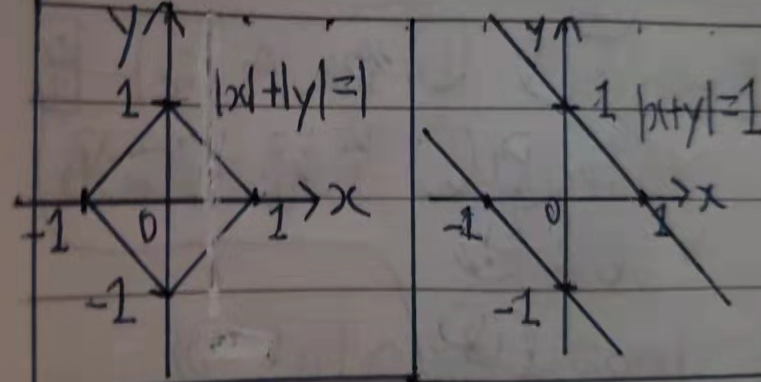
\includegraphics[scale=0.5]{img/20211023_calculusA_HW3_Fig_5.PNG}\newline
Since $\exists a$ s.t. $x=a$ and the each of the graphs have two intersections, neither are functions.
\subsection*{Problem 27.}
Find a formula for each function graphed.\newline
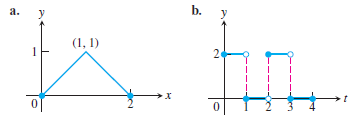
\includegraphics{./img/20211023_calculusA_HW3_Fig_1.png}
\subsection*{Solution 27.}
\begin{enumerate}[label=(\alph*)]
    \item $y=\left\{\begin{array}{cc}x,&0\leq x\leq 1\\2-x,& 1<x\leq 2\end{array}\right.$
    \item $y=\left\{\begin{array}{cc}2,&0\leq x< 1\lor 2\leq x<3\\0,& 1\leq x< 2 \lor 3 \leq x \leq 4\end{array}\right.$
\end{enumerate}
\section*{1.5}
\subsection* {Problem 50.}
The accompanying figure shows the graph of a function $g(t)$ with domain $[-4,0]$ and range $[-3,0]$. Find the domains and ranges of the following functions, and sketch their graphs.
\begin{center}
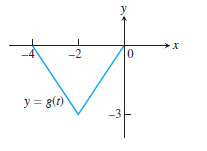
\includegraphics{./img/20211023_calculusA_HW3_Fig_2.png}
\end{center}
\[\begin{array}{cccccccc}\mathbf{a.}\,g(-t)&\mathbf{b.}\,-g(t)&\mathbf{c.}\,g(t)+3&\mathbf{d.}\,1-g(t)&\mathbf{e.}\,g(-t+2)&\mathbf{f.}\,g(t-2)&\mathbf{g.}\,g(1-t)&\mathbf{h.}\,-g(t-4)\end{array}\]
\subsection*{Solution 50.}


\begin{tabular}[b]{|c|c|c|p{100mm}|}
\hline
function&domain&range&graph\\
\hline
$g(-t)$&$[0,4]$&$[-3,0]$&\multirow{8}{*}{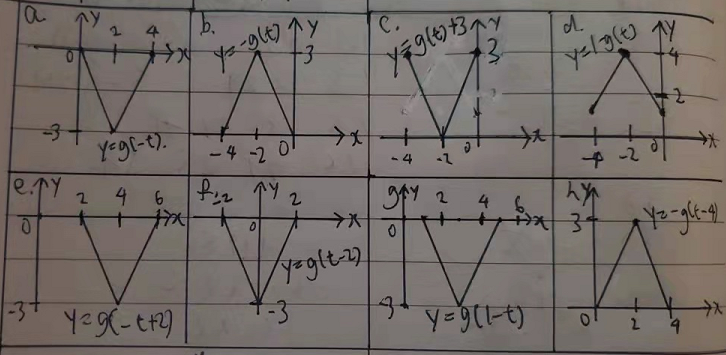
\includegraphics[scale=0.8]{img/20211023_calculusA_HW3_Fig_6.PNG}}\\[1.3ex]
\cline{1-3}
$-g(t)$&$[-4,0]$&$[0,3]$\\[1.3ex]
\cline{1-3}
$g(t)+3$&$[-4,0]$&$[0,3]$\\[1.3ex]
\cline{1-3}
$1-g(t)$&$[-4,0]$&$[1,4]$\\[1.3ex]
\cline{1-3}
$g(-t+2)$&$[2,6]$&$[-3,0]$\\[1.3ex]
\cline{1-3}
$g(t-2)$&$[-2,2]$&$[-3,0]$\\[1.3ex]
\cline{1-3}
$g(1-t)$&$[1,5]$&$[-3,0]$\\[1.3ex]
\cline{1-3}
$-g(t-4)$&$[0,4]$&$[0,3]$\\[1.3ex]
\hline
\end{tabular}
\subsection* {Problem 69.}
Graph the function $y=|x^2-1|$
\subsection*{Solution 69.}
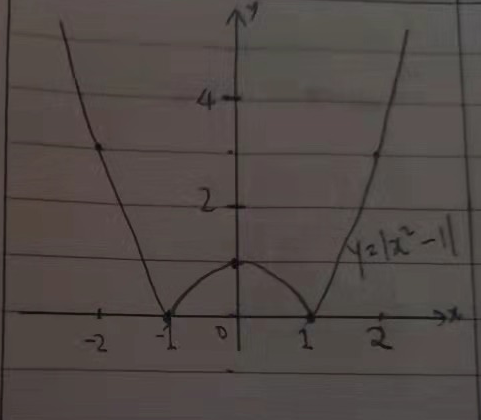
\includegraphics[scale=0.75]{img/20211023_calculusA_HW3_Fig_7.PNG}
\subsection* {Problem 79.}
Assume that $ƒ$ is an even function, $g$ is an odd function, and both $ƒ$ and $g$ are defined on the entire real line $\mathbb{R}$. Which of the following (where defined) are even? odd?\newline
\begin{tabular}{ccccccccc}
\textbf{a.}$fg$&\textbf{b.}$f/g$&\textbf{c.}$g/f$&
\textbf{d.}$f^2=ff$&\textbf{e.}$g^2=gg$&\textbf{f.}$f\circ g$&
\textbf{g.}$g\circ f$&\textbf{h.}$f\circ f$&\textbf{i.}$g\circ g$
\end{tabular}
\subsection*{Solution 79.}
$f(-x)=f(x),g(-x)=-g(x)$\newline
\begin{tabular}{|c|c|c|c|c|c|c|c|c|}
\hline
$fg$&$f/g$&$g/f$&$f^2=ff$&$g^2=gg$&$f\circ g$&$g\circ f$&$f\circ f$&$g\circ g$\\
\hline
odd&odd&odd&even&even&even&even&even&odd\\
\hline
\end{tabular}
\section*{1.6}
\subsection* {Problem 49.}
Find the value of $\sin^2{\frac{\pi}{12}}$
\subsection*{Solution 49.}
\[\sin^2{\frac{\pi}{12}}=\frac{1-\cos{\frac{\pi}{6}}}{2}=\frac{2-\sqrt{3}}{4}\]
\subsection* {Problem 53.}
Apply the law of cosines to the triangle in the accompanying figure to derive the formula for $\cos{(A-B)}$.
\begin{center}
    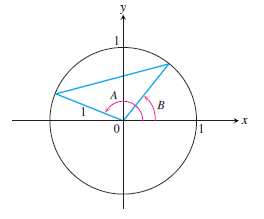
\includegraphics{img/20211023_calculusA_HW3_Fig_3.PNG}
\end{center}
\subsection*{Solution 53.}
Let $P_A=(\cos{A},\sin{A}),P_B=(\cos{B},\sin{B})$.\newline
On one hand,
\[|P_AP_B|^2=1^2+1^2-2(1)(1)\cos{(A-B)}=2-2\cos{(A-B)}\]
On the other hand,
\[|P_AP_B|^2=(\cos{A}-\cos{B})^2+(\sin{A}-\sin{B})^2\]
\[=\cos^2A-2\cos{A}\cos{B}+\cos^2B+\sin^2A-2\sin{A}\sin{B}+\sin^2B\]
\[=2-2\cos{A}\cos{B}-2\sin{A}\sin{B}\]
Thus,
\[2-2\cos{A}\cos{B}-2\sin{A}\sin{B}=2-2\cos{(A-B)}\Rightarrow \cos{(A-B)}=\cos{A}\cos{B}+\sin{A}\sin{B}\]
\subsection* {Problem 57.}
\textbf{The law of sines} The \textit{law of sines} says that if $a$,$b$ and $c$ are the sides of opposite the angles $A$, $B$ and $C$ in a triangle, then
\[\frac{\sin{A}}{a}=\frac{\sin{B}}{b}=\frac{\sin{C}}{c}\]
\begin{center}
    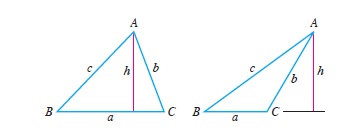
\includegraphics{img/20211023_calculusA_HW3_Fig_4.PNG}
\end{center}
Use the accompanying figures and the identity
$\sin(\pi-\theta)=\sin{\theta}$ if required, to derive the law.
\subsection*{Solution 57.}
Consider the area of that triangle, and denote $S_{\triangle ABC}$ as the area of $\triangle ABC$.\newline
Case $\triangle ABC$ is an acute triangle, $S_{\triangle ABC}=\frac{1}{2}ah=\frac{1}{2}ab\sin{C}$\newline
Case $\triangle ABC$ is an obtuse triangle, $S_{\triangle ABC}=\frac{1}{2}ah=\frac{1}{2}ab\sin{(\pi-C)}=\frac{1}{2}ab\sin{C}$\newline
Similarly, $S_{\triangle ABC}=\frac{1}{2}bc\sin{A}$, $S_{\triangle ABC}=\frac{1}{2}ca\sin{B}$.\newline
Hence, $\frac{1}{2}ab\sin{C}=\frac{1}{2}bc\sin{A}=\frac{1}{2}ca\sin{B}\Rightarrow \frac{\sin{A}}{a}=\frac{\sin{B}}{b}=\frac{\sin{C}}{c}$.
\end{document}